\subsection{The Impact of RNA-Binding on IFIT2-pIB Interaction} \label{subsec:The Impact of RNA-Binding on IFIT2-pIB Interaction}
\subsubsection{The Generation of Bovine IFIT2 RNA-Binding Mutant} \label{The Generation of Bovine IFIT2 RNA-Binding Mutant}
Using published data about hIFIT2 rna-binding mutant

Difficulty of using alpha-fold with IFIT2 due to the swap domain

Using SWISS-MODEL to predict bIFIT2 structure from published hIFIT2 structures

Alignment of both structures, assessment of electrostatic charges and establishment of residues to be mutated

Primer design and mutagenesis procedure based on published hIFIT2 RNA-binding mutant paper

\begin{figure}
    \centering
    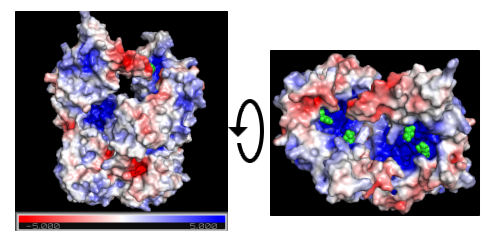
\includegraphics[width=1\linewidth]{10. Chapter 5/Figs/04. IFIT2-RNA binding mutant/01. structure.png}
    \caption[ifit2 mutant structure]{\textbf{ifit2 mutant structure.} Nascent bovine IFIT1 in the context of bRSV infection has been observed to localise with the respect of IB in three distinct spaces. We observed it either concentrated inside the central point of the IB structure, while having reduced signal on the inner IB edge, compared to the cytoplasm (top and bottom panels), being excluded from the IB structure (3rd panel), or colocalising on the inner edge of the IB structure while having reduced signal in the middle of the structure compared to cytoplasm, or the edge staining (2nd panel).}
    \label{fig:ifit2 mutant structure}
\end{figure}

\subsubsection{Bovine IFIT2 RNA-Binding Mutant and RSV pIBs} \label{Bovine IFIT2 RNA-Binding Mutant and RSV pIBs}
%bi2f24 + hnhp
Cell Line: VERO
Treatment: hNhP + bIFIT2-FLAG-RBM
Detecting magenta: exogenous bovine IFIT2 RBM
Detecting cyan: human pIB

In the second experiment we see consistent colocalization and/or inclusion of bovine IFIT2 RNA-binding mutant with human pseudo inclusion bodies.

\begin{figure}
    \begin{subfigure}{0.5\textwidth}
        \caption{}
        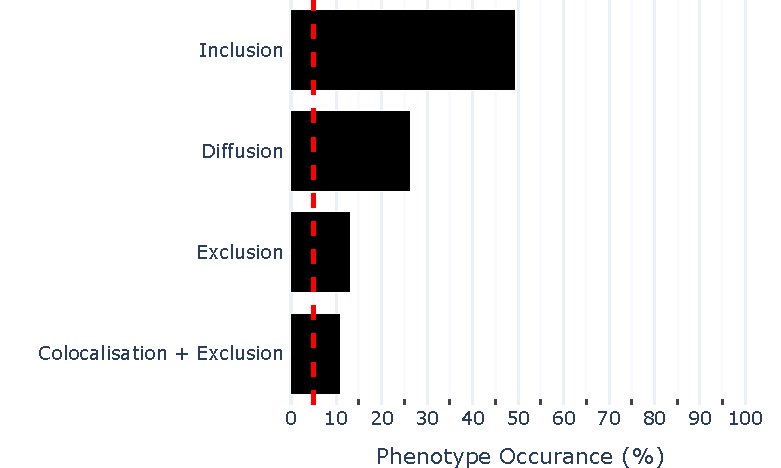
\includegraphics[width=1\linewidth]{10. Chapter 5/Figs/04. IFIT2-RNA binding mutant/02. pIB/01. bar_bi2f24_hnhp.pdf} 
    \end{subfigure}
    \begin{subfigure}{0.5\textwidth}
        \caption{}
        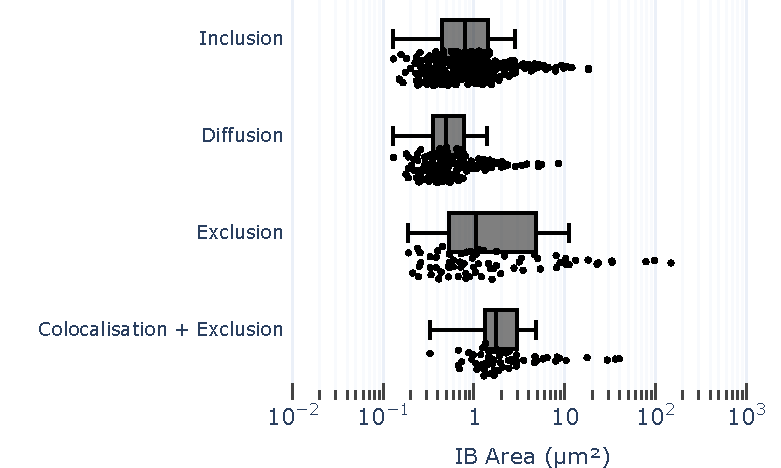
\includegraphics[width=1\linewidth]{10. Chapter 5/Figs/04. IFIT2-RNA binding mutant/02. pIB/02. box_bi2f24_hnhp.pdf}
    \end{subfigure}
    \caption[bi2f24 + hnhp plots]{\textbf{bi2f24 + hnhp plots.} Nascent bovine IFIT1 in the context of bRSV infection has been observed to localise with the respect of IB in three distinct spaces. We observed it either concentrated inside the central point of the IB structure, while having reduced signal on the inner IB edge, compared to the cytoplasm (top and bottom panels), being excluded from the IB structure (3rd panel), or colocalising on the inner edge of the IB structure while having reduced signal in the middle of the structure compared to cytoplasm, or the edge staining (2nd panel).}
    \label{fig:bi2f24 + hnhp plots}
\end{figure}

\begin{figure}
    \centering
    
\includegraphics[width=1\linewidth]{10. Chapter 5/Figs/00. placeholder.png}
    \caption[bi2f24 + hnhp]{\textbf{bi2f24 + hnhp.} Nascent bovine IFIT1 in the context of bRSV infection has been observed to localise with the respect of IB in three distinct spaces. We observed it either concentrated inside the central point of the IB structure, while having reduced signal on the inner IB edge, compared to the cytoplasm (top and bottom panels), being excluded from the IB structure (3rd panel), or colocalising on the inner edge of the IB structure while having reduced signal in the middle of the structure compared to cytoplasm, or the edge staining (2nd panel).}
    \label{fig:bi2f24 + hnhp}
\end{figure}

\begin{figure}
    \begin{subfigure}{0.5\textwidth}
        \caption{}
        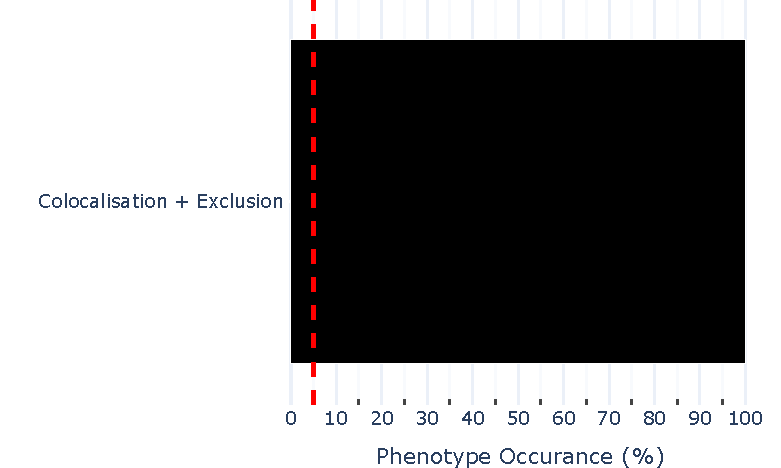
\includegraphics[width=1\linewidth]{10. Chapter 5/Figs/04. IFIT2-RNA binding mutant/02. pIB/04. bar_bi2f24_bnbp.pdf} 
    \end{subfigure}
    \begin{subfigure}{0.5\textwidth}
        \caption{}
        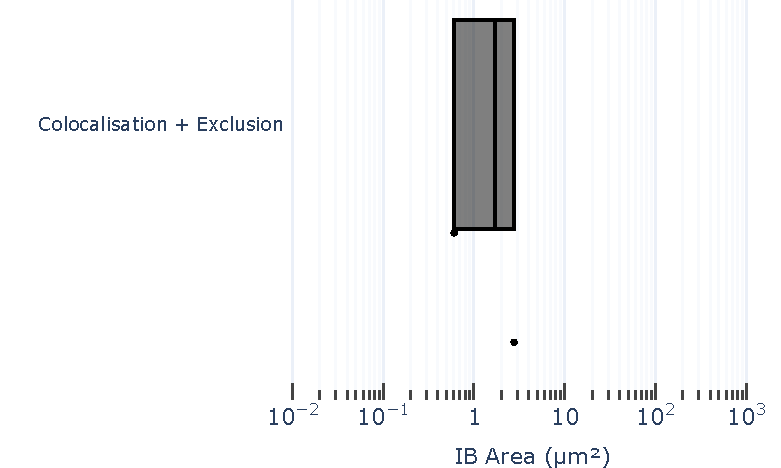
\includegraphics[width=1\linewidth]{10. Chapter 5/Figs/04. IFIT2-RNA binding mutant/02. pIB/05. box_bi2f24_bnbp.pdf}
    \end{subfigure}
    \begin{subfigure}{1\textwidth}
        \centering
        \caption{}
        
\includegraphics[width=1\linewidth]{10. Chapter 5/Figs/00. placeholder.png}
    \end{subfigure}
    \caption[bi2f24 + bnbp]{\textbf{bi2f24 + bnbp.} Nascent bovine IFIT1 in the context of bRSV infection has been observed to localise with the respect of IB in three distinct spaces. We observed it either concentrated inside the central point of the IB structure, while having reduced signal on the inner IB edge, compared to the cytoplasm (top and bottom panels), being excluded from the IB structure (3rd panel), or colocalising on the inner edge of the IB structure while having reduced signal in the middle of the structure compared to cytoplasm, or the edge staining (2nd panel).}
    \label{fig:bi2f24 + bnbp}
\end{figure}

\subsubsection{Summary}
We have described how bovine IFIT2 RNA-binding mutant was designed based on the published human IFIT2 RNA-binding mutant data (needs to be annotated more). Overexpression of bovine IFIT2 RNA-binding mutant yields cellular distribution and morphology similar to what was observed with overexpressing human IFIT2-FLAG, suggesting that the mutant proteins are not toxic to the cells. In the first experiment where we were looking at interaction between bovine IFIT2 RNA-binding mutant and human pseudo inclusion bodies we saw several phenotypes. We observed bovine IFIT2 RNA-binding mutant being excluded from small and big pIBs and pIB associated filamentous network, while fully or partially colocalising with other pIBs. In a subsequent experiment we observed only colocalization and inclusion formation. When assessing the interaction between bovine IFIT2 RNA-binding mutant and human pIBs formed using wild-type human RSV P and GFP-tagged human RSV N, we observed consistently in two experiments that bovine IFIT2 RNA-binding mutant colocalises to the pIB structures.